\section{Frontend}\label{sec:frontend}
The following section describes our user frontend and especially how we show data to the user in a compact manner.
The frontend is written in Angular using Angular Material library.
We devided the frontend in 5 parts.
The user can choose in a navigation bar between \textit{Dashboard}, \textit{Supplier}, \textit{Consumer}, \textit{Batteries} and \textit{Prices} view.
The views are decribed in the following subsections.

\subsection{Supplier and Consumer}
In the Supplier view the user can create, delete or manage supplier.
Creating, delete or manage consumer works equivalent so we will explain it only for supplier.

The interface for suppliers is shown in \cref{fig:suppliers}.
In the left side there is a navigation bar which shows all created supplier.
A user can add a new one using the \textit{plus} button under the suppliers, delete a specific supplier using the \textit{bin} button right to the supplier or manage the supplier clicking on it.
The main part of this page is the form with the user given data such as latitute, longitute or additional supplier specific needed data, e.g. rotator radius for wind turbines.
The kind of supplier can be chosen with the radio button above the form.
Due to angulars modularity it's easy to add more kinds of supplier in the future.
Next to the form is a map using angular leaflet openstreetmap API.
The nice part is that a user does not need to know the specific latitute or longitute to create supplier.
Clicking on the map adds a location point which can be exported easily to the form which allows the user to create suppliers at a specific place in the map.
Once created a supplier, it available in the navigation bar at the right.
Clicking on it shows all data already filled in the form and allows the user to change it during run time.


\begin{figure}[!h]
    \centering
    TODO%\includegraphics{}
    \caption{View to create, delete or manage suppliers}
    \label{fig:suppliers}
\end{figure}

\subsection{Batteries}
The batteries view is shown in \cref{fig:batteries}.
On the left side of the page there is the same kind of navigation bar we also used in the supplier and consumer pages to create, delete and manage batteries.
In the middle of the view there is also a form to set the batteries data.
The user can specify battery capacity, charge and discharge rates and efficiency as well as it's position.
The position can either set directly through the form or just like in the supplier or consumer view through the map using the export button.

\begin{figure}[!h]
    \centering
    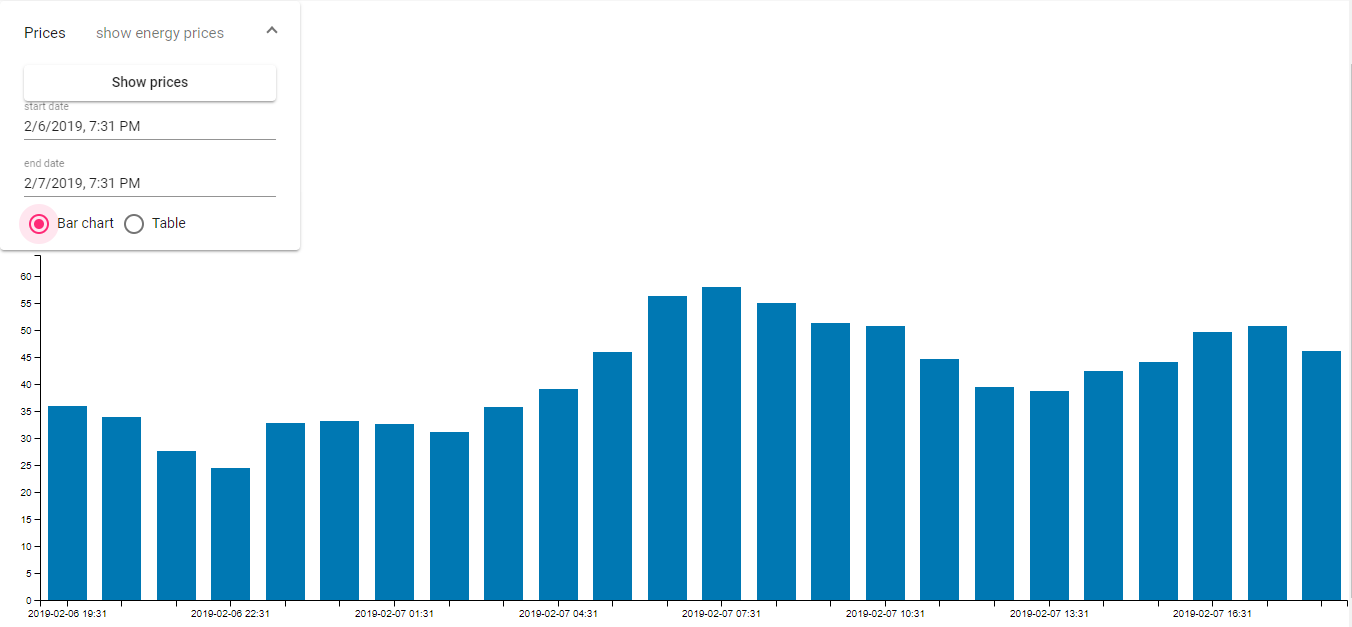
\includegraphics[width=1.00\textwidth]{../figures/batteries.PNG}
    \caption{View to create, delete or manage batteries}
    \label{fig:batteries}
\end{figure}



\subsection{Prices}
The prices view shows the energy prices for bidding zone DE-LU as table and bar chart.
The user can specify start and end date of the prices so he can take a look at the day-ahead prices as well as the past 5 days of the energy prices.
The page is shown in \cref{fig:prices}.

\begin{figure}[!h]
    \centering
    TODO%\includegraphics{}
    \caption{View show energy prices for specific time interval}
    \label{fig:prices}
\end{figure}

\subsection{Dashboard}
The most interesting view is the dashboard.
Here the user can take a look easily at different kinds of information in a compact manner.
The view is divided in two parts as shown in \cref{fig:dashboard}.

\begin{figure}[!h]
    \centering
    TODO%\includegraphics{}
    \caption{Dashboard view to show several kind of charts}
    \label{fig:dashboard}
\end{figure}

On the left side, the user can choose between the kinds of charts to get the chart he wants which is shown directly below.
On the right side the user can select the data which should be used in the chart.
Using the radiobuttons, the user can switch between \textit{All Demand and Supply}, \textit{All Demand}, \textit{All Supply} and \textit{Custom}, where he can choose each specific kind of data.
So it's possible for example to select wind turbines and homes to take a look if wind turbines can supply homes on their own.
In addition to this, we provide several templates the user can choose from.
Templates are predefined selections of data which are most likely interesting for a user, so he need less clicks to get the information he wants.
Which kind of charts the system currently supply is described in \cref{sec:charts}.

\subsection{Charts}\label{sec:charts}
Todo, describe kind of charts